\chapter{Shape of Nuclei}
\label{chapter-2}

\section{Nuclear Deformation}

\subsection{Collective coordinates}

The nuclear surface can be described through an expansion of the spherical harmonics with some time-dependent parameters as \emph{expansion coefficients}. The expression of the nuclear shape is given as \cite{greiner1996nuclear}:
\begin{align}
    R(\theta,\varphi,t)=R_0\left(1+\sum_{\lambda=0}^\infty\sum_{-\lambda}^\lambda\alpha_{\lambda\mu}(t)Y_\lambda^\mu(\theta,\varphi)\right)\ ,
    \label{nuclear-shape}
\end{align}
where $R$ denotes the nuclear radius. The radius is given as a function of spherical coordinates $\theta,\varphi$ and time. The radius of the spherical nucleus when all the expansion coefficients vanish is denoted by $R_0$. It is worth mentioning that the expansion coefficients $\alpha_{\lambda\mu}$ act as \emph{collective coordinates}, since the time-dependent amplitudes describe the vibrations of the nuclear surface.

% \subsection{Nuclear radius under rotation}

% To get a grasp at the physical meaning behind the deformation parameters that are used to describe the nuclear surface, it is instructive to see what happens when the system undergoes a rotation transformation.

% The function $R(\theta,\varphi)$ describes the original (non-rotated) nuclear shape. Rotating the system will result in the change of the angular coordinates $(\theta,\varphi)$ to $(\theta',\varphi')$, which will correspond to a new function $R'(\theta',\varphi')$. Moreover, both nuclear surfaces (i.e., the non-rotated and the rotated one) must hold the equality:
% \begin{align}
%     R'(\theta',\varphi')=R(\theta,\varphi)
% \end{align}

% The rotational invariance of $R$ employs that $R'(\theta,\varphi)$ must have the same functional form, but the expansion coefficients $\alpha_{\lambda\mu}$ must be rotated, meaning:
% \begin{align}
%     \sum_{\lambda\mu}\alpha_{\lambda\mu}'Y'_{\lambda\mu}(
%         \theta,\varphi)=\sum_{\lambda\mu}\alpha_{\lambda\mu}Y_{\lambda\mu}(
%             \theta,\varphi)\ . \label{nuclear_surface_equality}
% \end{align}

% Note that in Eq. \ref{nuclear_surface_equality}, the spherical harmonics $Y'_{\lambda\mu}$ are obtained via the usual rotation matrices. Finally, the invariance of Eq. \ref{nuclear-shape} is achieved if the set of parameters $\alpha_{\lambda\mu}$ transform similarly to a \emph{spherical tensor with angular momentum} $\lambda$ \cite{ring2004nuclear}, that is:
% \begin{align}
%     \alpha_{\lambda\mu}'=\sum_{\mu'}\mathcal{D}^{(\lambda)}_{\mu\mu'}\alpha_{\lambda\mu'}\ .
% \end{align}

% Besides the spherical tensor character, the collective coordinates also have the following properties (emerging from Eq. \ref{nuclear-shape}):
% \begin{itemize}
%     \item Complex Conjugation.
%     \begin{align}
%         Y^*_{\lambda\mu}(\theta,\varphi)&=(-1)^{\mu}Y_{\lambda-\mu}(\theta,\varphi), \\
%         \alpha^*_{\lambda\mu}&=(-1)^\mu\alpha_{\lambda-\mu}\ .
%     \end{align}
%     \item Parity - the coordinates $\alpha_{\lambda\mu}$ must undergo the same change of sign under a parity transformation as the spherical harmonics, in order to keep the invariance of the nuclear surface.
%     \begin{align}
%         (r,\theta,\varphi) &\xrightarrow[P]{}     (r,\pi-\theta,\pi+\varphi)\ \nonumber, \\
%         Y_{\lambda\mu}(\theta,\varphi) &\xrightarrow[P]{} Y_{\lambda\mu}(\pi-\theta,\pi+\varphi)=(-1)^\lambda Y_{\lambda\mu}(\theta,\varphi)\ .\nonumber
%     \end{align}
%     Therefore, the parity of the expansion coefficients are:
%     \begin{align}
%         \pi(\alpha_{\lambda\mu})=(-1)^\lambda\ .
%     \end{align}
% \end{itemize}

\subsection{Multipole deformations}

In the expansion of the nuclear surface defined by Eq. 
\ref{nuclear-shape}, the different values for $\lambda$ will determine different effects regarding the physical aspects of the nucleus. As such, the first values of $\lambda$ will be examined in terms of their physical meaning.
\begin{description}
    \item[Monopole mode] This corresponds to the first value of $\lambda=0$. This is the simplest mode of \emph{deformation} of a nuclear surface. Within this approximation, the spherical harmonic $Y_0^0$ is constant, which would imply that any non-vanishing values for $\alpha_{00}$ will correspond to the change in radius of the nucleus. This kind of excitation is also called \emph{breathing mode} of the nucleus \cite{greiner1996nuclear,bohr1998nuclear}. The energy required for this kind of excitation mode is very large, since it implies a compression of the nuclear matter. As a result, this mode is irrelevant in the low-lying excited spectra of atomic nuclei.
    \item[Dipole mode] Corresponds to $\lambda=1$. In reality, this type of mode does not manifest itself as a deformation of the nucleus, but rather as a shift of the nuclear center of mass.
    \item[Quadrupole mode] Excited mode that correspond to $\lambda=2$ are the most important collective excitations. The loss of axial symmetry, triaxial deformations, and other shape-specific features are direct consequences of quadrupole excitations.
    \item[Octupole mode] It corresponds to $\lambda=3$, representing the main asymmetric excitations of a nucleus with states of negative-parity. The specific shape of a nuclear system governed by octuple deformations is similar to that of a pear.
    \item[Hexadecapole deformations] Excitations with $\lambda=4$ are considered the highest angular momenta which can provide relevant information for the nuclear phenomena. Currently, there is no clear evidence for pure excitations with hexadecapole nature, however, these excitations seem to have a major role in the admixture to quadrupole excitations for the ground-state shape of heavy nuclei \cite{greiner1996nuclear}.
\end{description}

The multipole deformations for the cases $\lambda=1,2,3$ and $\lambda=4$ are shown in Fig. \ref{multipole-deformations}. Excitations with higher angular momentum than these have no practical application within the study of atomic nuclei. Moreover, one can also see that there is an intrinsic limitation on the maximal value of $\lambda$, which dictates the individual bumps of the surface (see Fig. \ref{multipole-deformations}). These bumps are described by the spherical harmonics $Y_\lambda^\mu$, and they decrease in size with increasing values of $\lambda$, but with the physical limitation given by the size of the nucleon diameter.
\begin{figure}
    \centering
    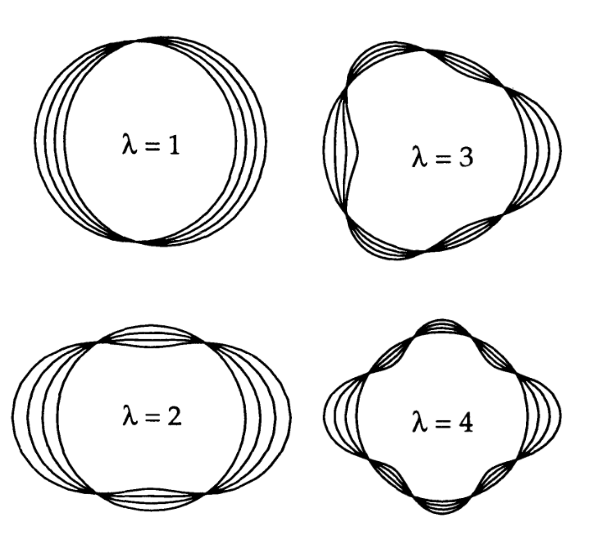
\includegraphics[scale=0.3]{Chapters/Figures/nuclearDeformation.png}
    \caption{Graphical representation of the first few modes of excitations of the nuclear surface. The figure is taken from Ref. \cite{greiner1996nuclear}.}
    \label{multipole-deformations}
\end{figure}

\section{Quadrupole Deformation}
\label{section:quadrupole-deformation}

One of the most important excitation modes (vibrational degrees of freedom) is the quadrupole deformation, corresponding to $\lambda=2$. In the case of pure quadrupole deformation, the nuclear surface will be given by the following expression:
\begin{align}
    R(\theta,\varphi)=R\left(1+\sum_{\mu=-2}^{2}\alpha_{2\mu}Y_2^\mu(\theta,\varphi)\right)\ . \label{quadrupole-surface}
\end{align}

From this expression, the term $\alpha_{00}$ is of second order in $\alpha_{2\mu}$ and it can be neglected further on. This term also reflects the conservation of volume \cite{greiner1996nuclear,ring2004nuclear}. The real and independent degrees of freedom from the above expression are: $\alpha_{20}$, the real and imaginary parts of $\alpha_{21}$, and the real and imaginary parts of $\alpha_{22}$. More insight in regard to the quadrupole shape of the nucleus can be achieved if one expresses $R$ in terms of Cartesian coordinates. The spherical harmonics will attain a new form, depending on the Cartesian components of the unit vector pointing in a direction defined by $(\theta,\varphi)$:
\begin{align}
    \xi=\sin\theta\cos\varphi\ ,\ \eta=\sin\theta\sin\varphi\ ,\ \zeta=\cos\theta\ ,
\end{align}
with the condition $\xi^2+\eta^2+\zeta^2=1$. With the expressions of the spherical harmonics as functions of $(\xi,\eta,\zeta)$, the nuclear radius will change accordingly. A relationship between the Cartesian components and the spherical ones for the deformation can be also obtained if all coefficients $\alpha_{2\mu}$ are written as functions of $\alpha_{ij}$ (with $i,j=\xi,\eta,\zeta$). Since the Cartesian deformations give the stretch/contraction of the nucleus in a given direction, a first interpretation of the physical meaning behind the parameters $\alpha_{2\mu}$ can be established:
\begin{itemize}
    \item $\alpha_{20}$: describes the stretching of the $z$ axis with respect to the $y$ and $x$ axes.
    \item $\alpha_{2-2}$ and $\alpha_{22}$: give the relative length of the $x$ axis compared to the $y$ axis. Moreover, it also gives the oblique deformation in the $x-y$ plane.
    \item $\alpha_{2-1}$ and $\alpha_{21}$: describe an oblique deformation, but with respect to the $z$ axis.
\end{itemize}

With the set of parameters defined above, the shape and orientation of the nucleus can have arbitrary values (the coefficients $\alpha_{2\mu}$ are mixing the shape and orientation), making the parametrization somewhat problematic. In order to fix that, the geometry can be changed if one considers the \emph{principal axis system}
% (the PA reference system is a coordinate system in which the moments of inertia associated with the nucleus are diagonal). 
When using this reference frame, the number of parameters is still unchanged, however their physical significance becomes clearer. By denoting the new coordinate system with primed letters, the nuclear radius will be described as a function $R=R(\xi',\eta',\zeta')$, with the conditions that $\alpha'_{ij}=0\ ,\ i\neq j$. The condition will further imply that the newly expressed parameters ($\alpha'_{2\mu}$) have the following form:
\begin{align}
    \alpha'_{2 \pm 1}&=0\ , \nonumber \\
    \alpha'_{2 \pm 2}&\equiv a_2\ , \nonumber \\
    \alpha'_{20}&\equiv a_0\ ,
\end{align}
where the conveniently denoted terms $a_2$ and $a_0$ depend on the Cartesian components $\alpha_{\xi,\xi}\ ,\ \alpha_{\eta,\eta}\ ,\ \alpha_{\zeta,\zeta}$. From this set of equations the physical significance of the five real and independent parameters is as follows:
\begin{itemize}
    \item $a_0$ is indicating the stretch of $z'$ axis w.r.t. the $x'$ and $y'$ axes.
    \item $a_2$ is indicating the asymmetry between the lengths of $x'$ and $y'$ axes, respectively.
    \item the three \emph{Euler angles} $\mathbf{\Theta}=(\theta_1,\theta_2,\theta_3$ that determine the orientation of the PA system $(x',y',z')$ with respect to the laboratory-fixed frame $(x,y,z)$.
\end{itemize}

The advantage in working within this coordinate system is clearly emphasized: rotation and shape vibration degrees of freedom are completely separated. A change in the Euler angles will emerge as a pure rotation of the nucleus, while a change in shape will be affected exclusively by the $a_0$ and $a_2$ parameters. If $a_2=0$, then the nucleus has is symmetric around the $z$-axis (equal lengths along the $x$ and $y$ directions). Another way of describing the excitations of quadrupole type is to adopt the parameters introduced by Bohr in Ref. \cite{bohr1954rotational}. These two parameters can be viewed as a set of polar coordinates in the space generated by $a_0$ and $a_2$, namely:
\begin{align}
    a_0&=\beta_2\cos\gamma\ , \nonumber \\
    a_2&=\frac{1}{\sqrt{2}}\beta_2\sin\gamma\ ,
    \label{bohr-deformation-params}
\end{align}
where the numeric factor $1/2$ was added such that the following relation holds true:
\begin{align}
    \sum_\mu\left|\alpha_{2\mu}\right|^2=\sum_\mu\left|\alpha'_{2\mu}\right|^2=a_0^2+2a_2^2=\beta_2^2\ .
    \label{quadrupole-param-sum}
\end{align}

It is worth mentioning that Eq. \ref{quadrupole-param-sum} is rotationally invariant, having the same value in the laboratory and the principal axes systems. Now that the shape of the nucleus (i.e., the nuclear surface radius $R$) can be described consistently with via the parameters defined in Eq. \ref{bohr-deformation-params}, one can calculate the stretching of the nuclear radius along any of the directions is given in terms of $(\beta,\gamma)$ as follows:
\begin{align}
    \delta R_k=\sqrt{\frac{5}{4\pi}}\beta\cos(\gamma-\frac{2\pi k}{3})\ .
    \label{axes-stretching}
\end{align}

\subsection{Axial quadrupole deformations}

Using this set of new coordinates, the expression of the nuclear radius for axially quadrupole-deformed nuclei is given as:
\begin{align}
    R(\theta,\varphi)=R_0\left(1+\beta_2 Y_2^0(\theta,\varphi)\right)\ ,
    \label{quadrupole-radius}
\end{align}
where the parameter $\beta_2$ is called the \emph{quadrupole deformation parameter}, and its value dictates whether the nucleus is \emph{oblate} (i.e., a flattened sphere), \emph{prolate} (i.e., an elongated sphere, like a rugby ball), or \emph{spherical}. The nuclear shapes that are characterized only by $\beta_2$ (i.e., $\gamma=0$) have shapes that correspond to spheroids. These shapes are axially symmetric, meaning that they only have one deformed axis. For the axially-symmetric quadrupole deformations, the parameter $\beta_2$ can be related to the axes of the spheroid via Eq. \ref{axes-stretching}.
\begin{figure}
    \centering
    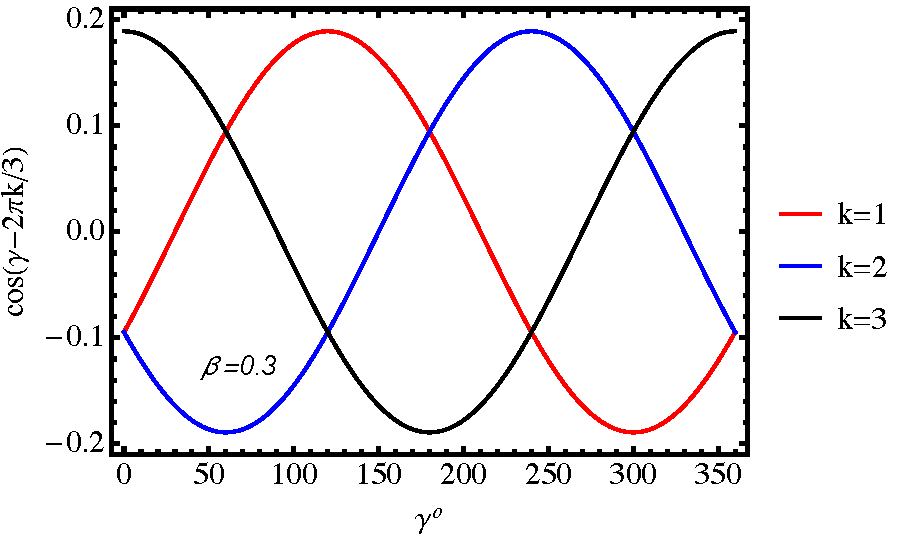
\includegraphics[scale=0.7]{Chapters/Figures/nuclear-radius-elongation.pdf}
    \caption{Graphical representation with the stretching of the nuclear axes $\delta R_k\ ,\ k=1,2,3$, corresponding to the increase in axis lengths along the $x$, $y$, and $z$ directions. The representation used an arbitrary value $\beta_2=0.3$. Figure was reproduced according to the calculations done in Ref. \cite{greiner1996nuclear}.}
    \label{nuclear-radius-elongation}
\end{figure}

Taking a look at Fig. \ref{nuclear-radius-elongation}, one can see the variations of the three axes with respect to $\gamma$. When $\gamma=0^\circ$, the nucleus is elongated along the $z'$ axis, but the $x'$ and $y'$ axes are identical (the prolate case). As $\gamma$ increases, the $x'$ axis grows, while the other two axes decrease in size, making a region with \emph{triaxial shapes}. Symmetry is reached again at $\gamma=60^\circ$, where $x'$ and $z'$ axes are equal but longer than $y'$ axis, making the nucleus look like a flattened shape (the oblate case). This pattern is repeated every $\gamma=60^\circ$, where alternating prolate/oblate shapes occur. It is possible to summarize the various nuclear shapes with a graphical representation within in the $(\beta,\gamma)$ plane. In Fig. \ref{beta-gamma-plane} one can the oblate shapes at $\gamma=60^\circ,180^\circ,300^\circ$, while prolate shapes appear at $\gamma=0^\circ,120^\circ,240^\circ$.
\begin{figure}
    \centering
    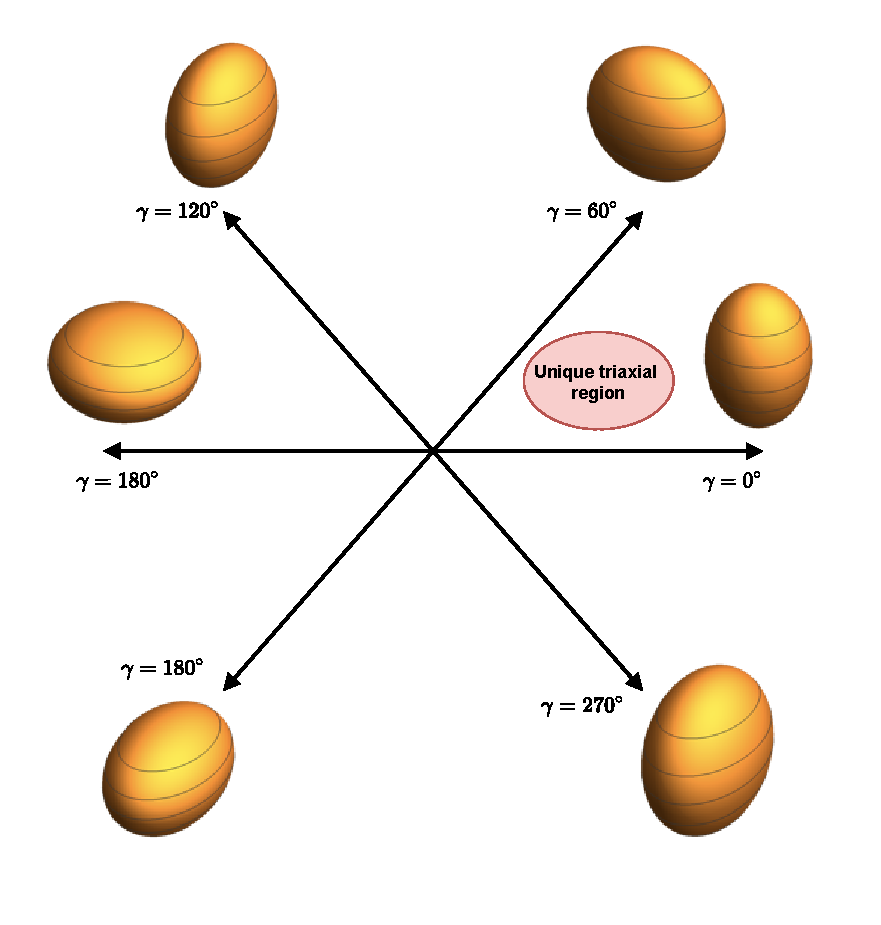
\includegraphics[width=0.99\textwidth]{Chapters/Figures/beta_gamma_plane.pdf}
    \caption{Beta-gamma plane divided into six regions. The first part, delimited from $\gamma=0^\circ$ to $\gamma=60^\circ$ can be considered as the representative one, while the others can be reproduced from this interval.}
    \label{beta-gamma-plane}
\end{figure}

\subsection{Non-Axial quadrupole deformations}

Besides the nuclei characterized by a \emph{spheroidal} shape where two of the principal axes are equal, there are also \emph{triaxial} (or non-axial) nuclei. The triaxial shapes are defined by the $\gamma$ degree of freedom: a parameter which dictates the asymmetry between the three axes of the nucleus (e.g., it describes a stretching along an axis that is perpendicular to the symmetry axis). The nuclear radius for the axially-asymmetric quadrupole deformations is given by:
\begin{align}
    R(\theta,\varphi)=R_0\left(1+\beta_2\cos\gamma Y_2^0(\theta,\varphi)+\frac{1}{\sqrt{2}}\sin\gamma(Y_2^2(\theta,\varphi)+Y_2^{-2}(\theta,\varphi))\right)\ ,
    \label{non-axial-quadrupole}
\end{align}
which is different from Eq. \ref{quadrupole-radius}. The values $\gamma=0^\circ$ and $\gamma=60^\circ$ correspond to symmetric prolate and oblate shapes, respectively. Between these values, the triaxial region exist, with \emph{maximal triaxiality} reached at $\gamma=30^\circ$. The deformation parameters $(\beta,\gamma)$ are also called the Hill-Wheeler set \cite{wong2008introductory}. In Eq. \ref{non-axial-quadrupole}, the spherical harmonics are expressed as follows:
\begin{align}
    Y_2^0(\theta,\varphi)&=\frac{1}{4}\sqrt{\frac{5}{\pi}}\left(3\cos^2\theta-1\right)\ , \nonumber\\
    Y_2^2(\theta,\varphi)&=\frac{1}{4}e^{2i\varphi}\sqrt{\frac{15}{2\pi}}\sin^2\theta\ ,\nonumber\\
    Y_2^{-2}(\theta,\varphi)&=\frac{1}{4}e^{-2i\varphi}\sqrt{\frac{15}{2\pi}}\sin^2\theta\ ,
\end{align}
and substituting these terms in $R(\theta,\varphi)$, the structure Eq. \ref{non-axial-quadrupole} will become \cite{andersson1976nuclear,bohr1998nuclear}:
\begin{align}
    R(\theta,\varphi)=R_0\left[1+\sqrt{\frac{5}{16\pi}}\beta\left(\cos\gamma(3\cos\theta^2-1)+\sqrt{3}\sin\gamma\sin\theta^2\cos2\varphi\right)\right]\ .
\end{align}

Regarding the nuclear shapes that were described in Fig. \ref{beta-gamma-plane}, the redundancies of the $(\beta,\gamma)$ variables are:
\begin{itemize}
    \item for $\beta_2>0$ the nucleus is \emph{prolate} for $\gamma=0^\circ,120^\circ,240^\circ$.
    \item for $\beta_2>0$ the nucleus is \emph{oblate} for $\gamma=60^\circ,180^\circ,300^\circ$.
    \item for $\gamma=0^\circ,180^\circ$, the symmetry axis is the $z$-axis of the intrinsic frame
    \item for $\gamma=120^\circ,300^\circ$, the symmetry axis is the $x$-axis of the intrinsic frame
    \item for $\gamma=60^\circ,240^\circ$, the symmetry axis is the $y$-axis of the intrinsic frame
\end{itemize}

\subsection{Lund Convention}
\label{subsection:lund-convention}

The so-called Lund convention \cite{andersson1976nuclear} somewhat solves this repetitiveness, by selecting a rotational axis according to the set of rules described below:
\begin{itemize}
    \item The quadrupole deformation parameter $\beta_2$ is always positive: $\beta_2\geq 0 $
    \item The rotation around the smallest axis ($s$-axis) implies the constraint on the triaxiality parameter $0^\circ\leq\gamma\leq60^\circ$.
    \item The rotation around the longest axis ($l$-axis) implies the constraint on the triaxiality parameter $-120^\circ\leq\gamma\leq-60^\circ$.
    \item The rotation around the medium/intermediate axis ($i$-axis) implies the constraint on the triaxiality parameter $-60^\circ\leq\gamma\leq 0^\circ$.
\end{itemize}

% Fig. \ref{lund-convention-graph} aims at depicting the mechanism behind the Lund convention. The graphical representations organized in Table \ref{table-ellipsoidal-shapes} show the possible nuclear shapes, depending on the number of deformation axes; namely, if there is only one deformation axis, then the nuclear shape is \emph{axial-symmetric} (oblate or prolate) and if there are two deformation axes, then the nucleus is \emph{triaxial} (axially-asymmetric). 
% \begin{figure}
%     \centering
%     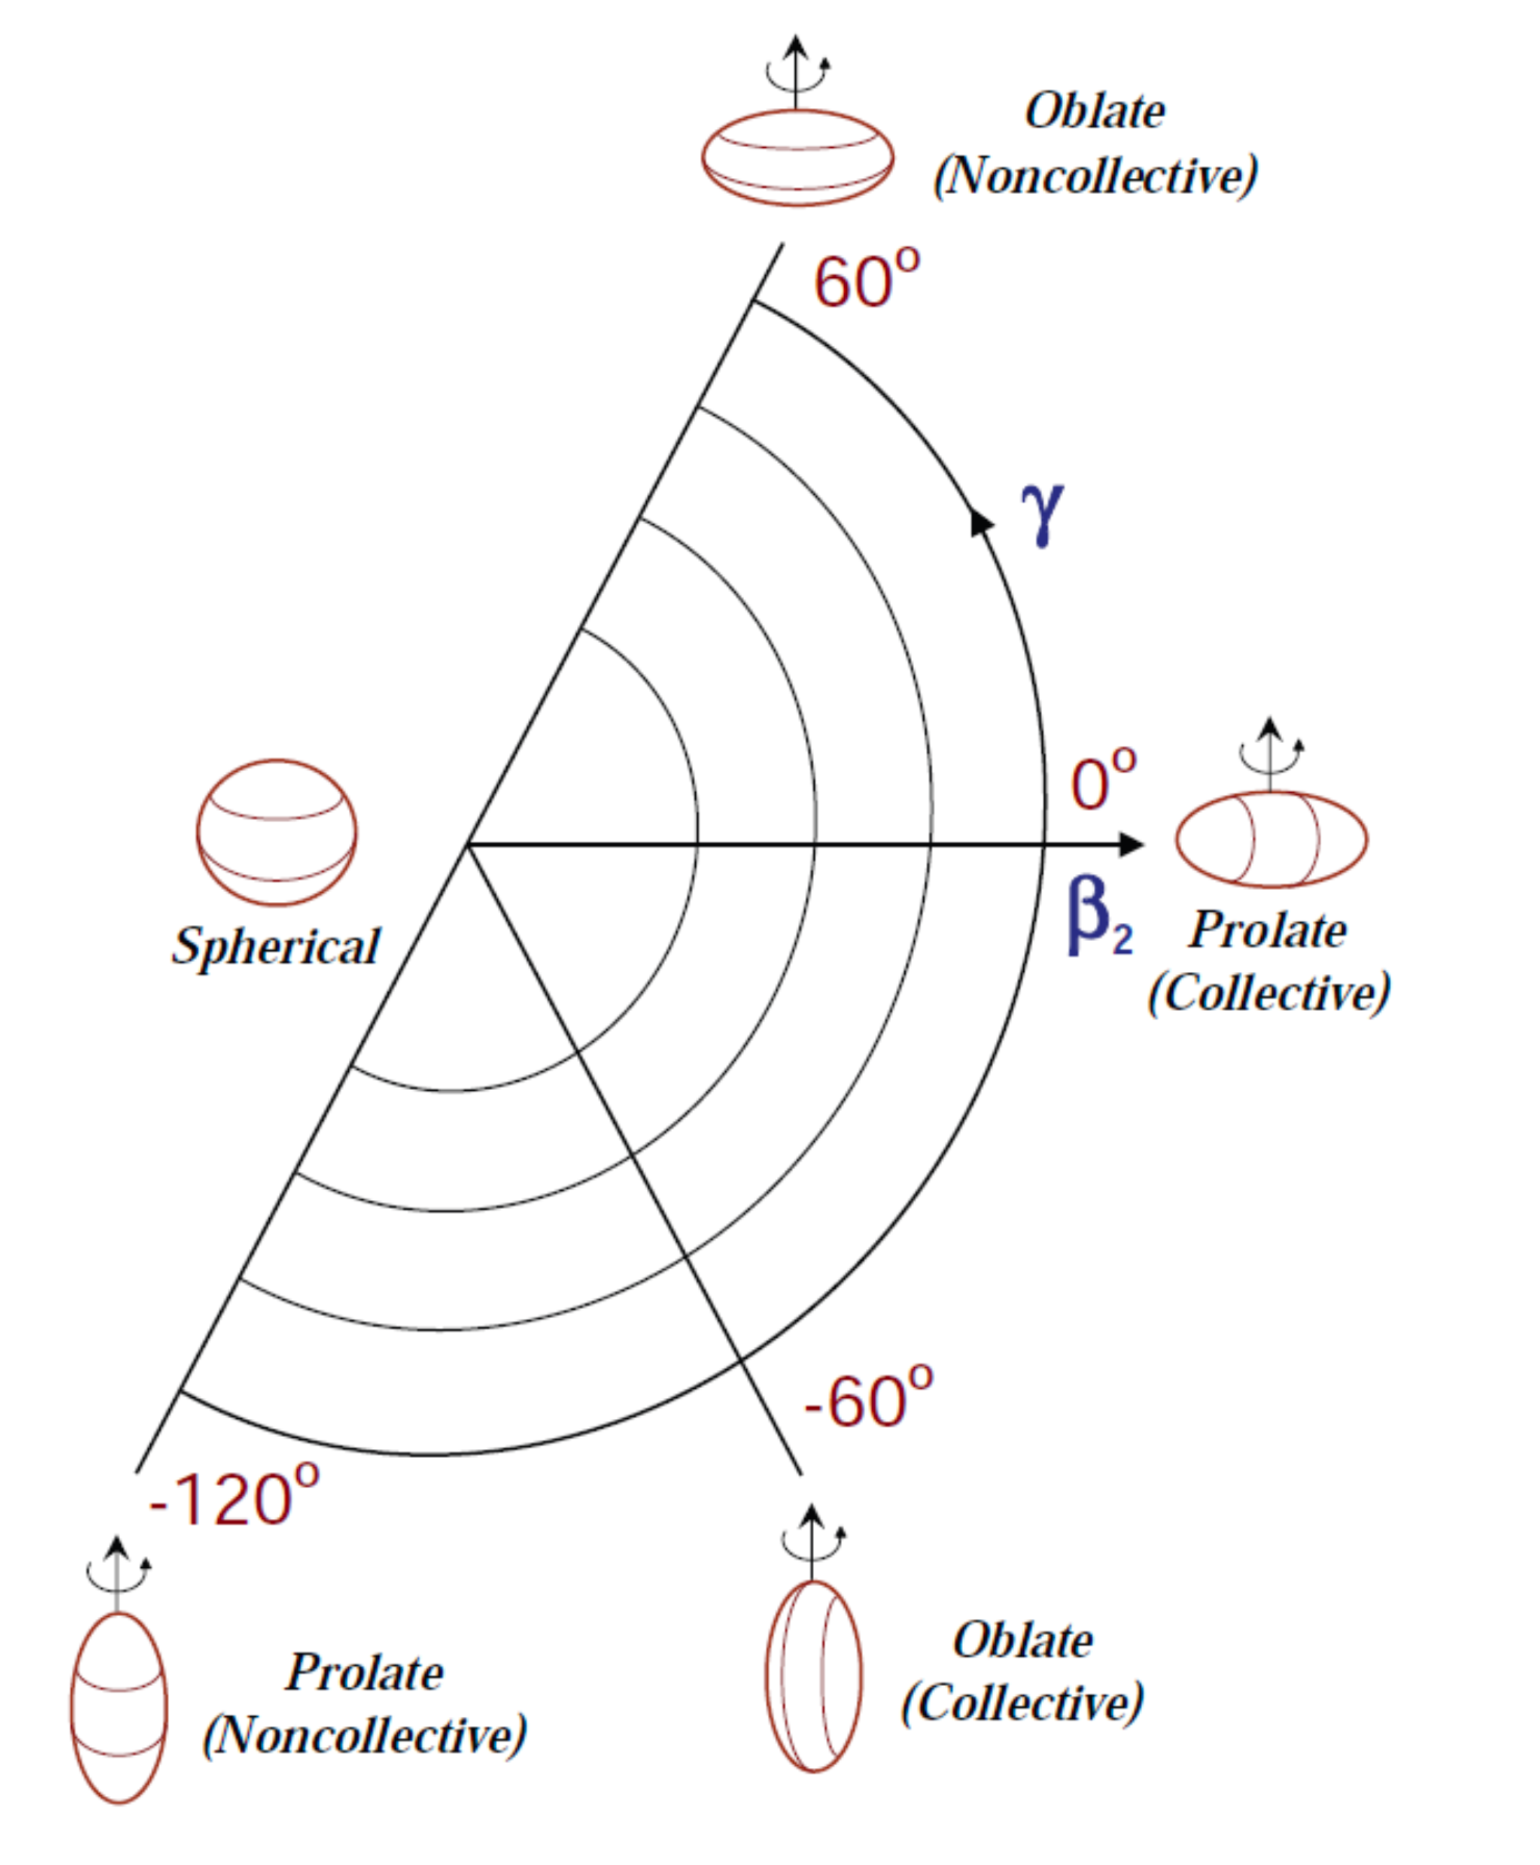
\includegraphics[scale=0.3]{Chapters/Figures/lund-convention-plot.pdf}
%     \caption{Representation of the nuclear shapes in the $(\beta,\gamma)$ plane, using the Lund convention \cite{andersson1976nuclear} previously discussed. The figure was taken from the work of Matta \cite{matta2017exotic}.}
%     \label{lund-convention-graph}
% \end{figure}
% \begin{table}
%     \centering
%     \begin{tabular}{|c|c|c|c|}
%         \hline 
%         \multicolumn{4}{|c|}{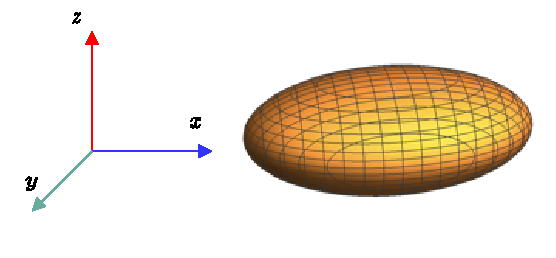
\includegraphics[scale=0.7]{Chapters/Figures/tabular_ellipse.pdf}}\\ \hline 
%         Shape    & \begin{tabular}[c]{@{}c@{}} n.o.\\ deformed axes\end{tabular} & Side view ($zx$-plane) & Top view ($yx$-plane) \\ \hline
%         Prolate  & 1                                                              &   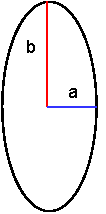
\includegraphics[scale=0.7]{Chapters/Figures/ellipse_prolate_1.pdf}   &     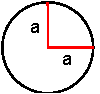
\includegraphics[scale=0.7]{Chapters/Figures/ellipse_prolate_2.pdf}      \\ \hline
%         Oblate   & 1                                                              &   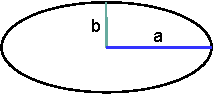
\includegraphics[scale=0.7]{Chapters/Figures/ellipse_oblate_1.pdf}    &     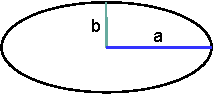
\includegraphics[scale=0.7]{Chapters/Figures/ellipse_oblate_2.pdf}       \\ \hline
%         Triaxial & 2                                                              &   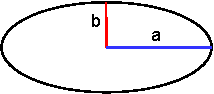
\includegraphics[scale=0.7]{Chapters/Figures/ellipse_triaxial_1.pdf}  &     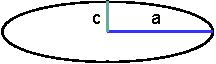
\includegraphics[scale=0.7]{Chapters/Figures/ellipse_triaxial_2.pdf}      \\ \hline
%         \end{tabular}
%     \caption{Deformed ellipsoidal shapes of the nuclei. A generic ellipsoid is shown at the top of the table. The parameters $a$, $b$, and $c$ represent lengths of differing magnitude of the nuclear ellipsoid.}
%     \label{table-ellipsoidal-shapes}
% \end{table}

\subsubsection{Alternative description of the quadrupole deformation}

Considering the Lund convention and the Eq. \ref{axes-stretching}, one can re-write the set of stretching values as follows:
\begin{align}
    \frac{R_x-R_0}{R_0}&=\sqrt{\frac{5}{4\pi}}\beta_2\cos\left(\gamma-\frac{2}{3}\pi\right)\ , \\
    \frac{R_y-R_0}{R_0}&=\sqrt{\frac{5}{4\pi}}\beta_2\cos\left(\gamma-\frac{4}{3}\pi\right)\ , \\
    \frac{R_z-R_0}{R_0}&=\sqrt{\frac{5}{4\pi}}\beta_2\cos\gamma. \\
\end{align}

For the axially symmetric deformation (i.e., $\gamma=0$), the quadrupole parameter $\beta_2$ can be derived as follows:
\begin{align}
    \beta_2=\frac{4}{3}\sqrt{\frac{\pi}{5}}\frac{R_z-R_x}{R_0}\ ,
\end{align}
where $R_z-R_x$ is the difference between the major ($R_z$) and minor ($R_x$) axes of the ellipsoid. This equation for $\beta_2$ shows how for oblate deformations, $\beta_2<0$ (implying that $R_z<R_x$), while for prolate deformations $\beta_2>0$ (implying that $R_z>R_x$). Within literature, usual values for $\beta_2$ range from 0.2 - 0.3 (known as \emph{normal deformation}) to 0.4 - 0.6 (known as strong or \emph{superdeformation}). Very often, an alternative description of the nuclear deformation is used in terms of the parameter $\epsilon_2$ that relates to $\beta_2$ via the formula \cite{casten2000nuclear}:
\begin{align}
    \epsilon_2\approx=\frac{R_z-R_x}{R_0}=\frac{3}{4}\sqrt{\frac{5}{\pi}}\beta_2=0.946\beta_2\ .
    \label{epsilon-beta-relation}
\end{align}

In this chapter, the concept of nuclear shape was introduced through the description of a nuclear radius parametrized in terms of collective coordinates and spherical harmonics, as per Eq. \ref{nuclear-shape}. The relevant excitations of the nuclear surface were emphasized, and the importance of $\lambda=2$ mode was illustrated in Section \ref{section:quadrupole-deformation}. A set of deformation parameters that describe the nuclear shape in terms of elongation and asymmetry, i.e., $\beta$ and $\gamma$ are also attained by means of geometrical transformations from Eq. \ref{bohr-deformation-params}. These two parameters are crucial quantities for the development of the theoretical models that will be presented in the later chapters.

% \subsection{Nuclear Shapes and Softness}

% A discussion about the implications of the nuclear shapes in terms of some specific phenomena is necessary. Indeed, the shell-model (which will be briefly discussed in the next chapter) considers the motion of the individual nucleons, that are \emph{confined} in nucleonic orbitals, where each nucleon will occupy an orbit with a quantized value of angular momentum. The interpretation of the gamma-ray spectra of different nuclei can be properly described through the excitations if individual nucleons between different orbits, but only for nuclei that are near closed shells. 

% Unfortunately, the same cannot be said about nuclei that lie far from a shell closure, where tools like \emph{Collective Model} - C.M. \cite{bohr1998nuclear} help understand the properties of these nuclei. One can see that any additional nucleon to the closed shells will imply a departure from the spherical view of a nucleus, with deformations along one of the axis of that nucleus. With the help of C.M., the energy spectrum of many nuclei can be understood and described in terms of 1) a rotation around an axis that is perpendicular to the deformation axis, but also in terms of a 2) motion of the nucleus as a whole (i.e., collective behavior) in tandem with one coming from a single nucleon (i.e., single-particle behavior).

% As an example, nuclei in the region $N=82$ were extensively studied, and the properties of a given nuclide are not only determined by the specific orbital occupied by valence nucleons (e.g., proton orbitals such as $s_{1/2}$, $h_{11/2}$ or neutron orbitals such as $f_{7/2}$, $h_{9/2}$), but also the proportion of each shell that is filled with protons and neutrons, respectively. The nuclei in this closed shell $N=82$ region are considered as perfect examples of evolutions from the single-particle motion, and the evolution to a collective behavior can be emphasized around the \emph{midshell} at $N=104$. 

% These midshell nuclei have a deformation that is present along only one axis: \emph{axially symmetric}. Every orbital will cause the nucleus to change its shape towards either a prolate or an oblate one. The change in prolate/oblate type of deformation will depend on the value of the quadrupole moment \cite{lewis2019lifetime}, quantity used to evaluate the so-called Nilsson levels \cite{ragnarsson2005shapes} (a detailed discussion about the Nilsson orbitals will be made in the following chapter), or Nilsson diagrams: single-particle energies as a function of nuclear deformation. The slope of a Nilsson level is related to the expectation value of the quadrupole moment, via the expression \cite{andersson1976nuclear}:
% \begin{align}
%     \frac{d e_k}{d\beta}=-\bra{j}q\ket{j}\, 
% \end{align}
% where $e_k$ represents the energy of the single-particle state $\ket{j}$, $\beta$ is the deformation, and $q$ is the quadrupole operator. Each nucleon that occupies an orbit with a given slope will contribute to an overall deformation: one nucleon that occupies a downward sloping orbital which for positive $\beta$ will drive the nucleus to a prolate shape, while the other type of nucleon that occupies an upward sloping orbital will drive the nucleus to an oblate shape. The competition between these two polarizing effects will result in the axial asymmetry.

% In triaxial nuclei (\emph{axially-asymmetric}), a number of low-lying nuclear configurations can exist, leading to different shapes. When the nucleus has a dynamic degree of triaxiality (via the $\gamma$ deformation parameter), it is said to be a $\gamma$-\emph{soft nucleus}. 

% The $\gamma$-soft nuclei tend to exist when both the protons and neutrons occupy the top and bottom of their shells, respectively. The opposite also holds true \cite{chen2014collective}. The conditions for $\gamma$-soft nuclear deformations are realized, for example, in $N \approx 90$ nuclei, where the Fermi surfaces are located near the top of the proton shell ($h_{11/2}$) and bottom of the neutron shell ($i_{13/2}$).

% It is interesting that a single nucleus does not necessarily holds a single fixed shape. If the potential energy surface (PES) is relatively flat with respect to the triaxiality parameter $\gamma$ (meaning that there is no constrain with regards to the minimum value of $\gamma$), the shape can oscillate within an interval of deformation. Such a feature characterizes the $\gamma$-softness of the nucleus itself.